\section{Stream Mining}
\label{Theory::StreamMining}

Data stream mining is a relatively new field. Even though its theoretical foundation is based in well-established statistical and computational approaches, it has not been until recent years that this research area has experimented a great growth in interest.

The main problem when dealing with streaming data is the high throughput of data being analyzed, under computational resources constraints. Variable data rates is another problem that has to be addressed too. Once these problems are resolved, the same kind of data mining analysis as in the case of batch data processing are available: classification, regression or clustering tasks, as well as outlier detection and recommendation systems. We will not cover these techniques here, because they are not related to this project, by themselves. Instead, we will have a look at some different stream mining solutions, because their working principles do affect the way the project’s algorithms will be implemented.

\subsection{Stream mining approaches}
\label{Theory::StreamMining::Approaches}

Solutions provided in this field can be categorized into \textit{data-based} and \textit{task-based} ones~\citep{Gaber:MiningDataStreamsReview}, depending on their approach.

\subsubsection*{Data-based stream mining solutions}

The idea behind these solutions is to use a subset of the original dataset to perform the required analyses. Diverse techniques that have been used in this sense can further be split into two more categories:

\begin{itemize}
	\item \textbf{Sampling methods:} either by randomly picking samples of the data stream or by randomly selecting chunks (subsets) of the stream, sampling methods discard part of the incoming data, while performing the knowledge discovery processes with the sampled data. The main problem with this approach is that is hard to know when to pick a sample or which records should be stored, because there is no previous knowledge of the dataset size or its information structure.

	\item \textbf{Summarizing methods:} they use aggregated data or calculated statistical measures (that are continuously recalculated) to provide the information needed for the data mining algorithms. In this case, it is the loss of information and accuracy and the inability to control data distribution fluctuations what renders these methods not so usable as it was desired.
\end{itemize}

\begin{figure}
\centering
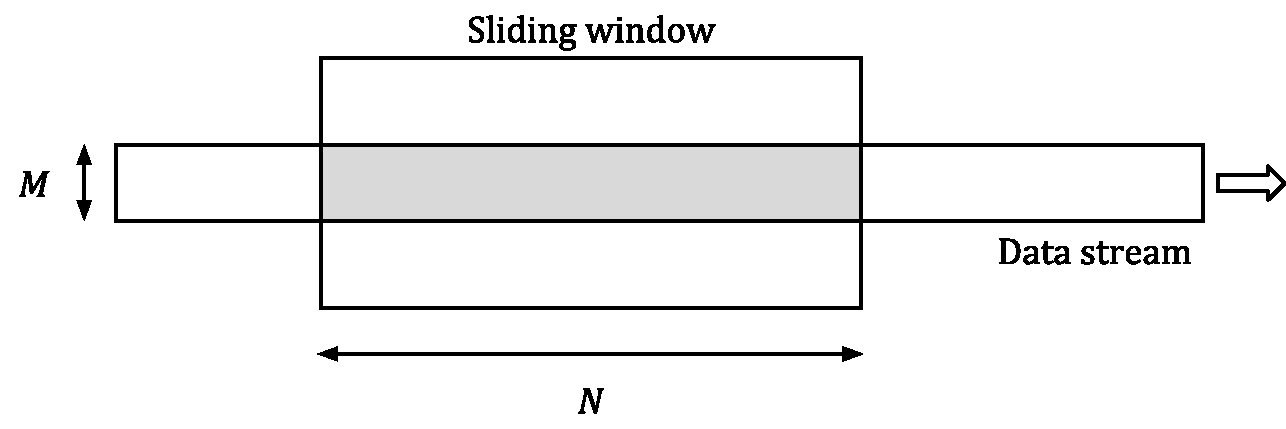
\includegraphics[width=0.9\linewidth]{figures/sliding-window.pdf}
\caption[Sliding window based stream processing.]{Processing a data stream using a \textit{sliding window} approach. In the figure, $N$ is the \textit{size} of the sliding window, in terms of the number of samples of the stream being stored, whereas $M$ is the number of \textit{attributes} of the samples in the stream.}
\label{fig:sliding-window}
\end{figure}

\subsubsection*{Task-based stream mining solutions}

The solutions that fall into this category are based not on performing data transformations, but on changing the data mining methods to enable their use on data streams.

\begin{itemize}
	\item \textbf{Approximation algorithms:} these are a kind of algorithms that are designed to solve computationally hard problems, by giving an approximate result. Instead of computing exact solutions, they just guarantee a certain error bound. The problem with these methods is, again, the high received data throughput, which they cannot cope as well. Additional tooling is therefore needed if one wishes to use them.

	\item \textbf{Sliding window method:} this method, a common pattern in many online\footnote{In computer science, an \textit{online algorithm} is one that can process its input piece-by-piece in a serial fashion, i.e., in the order that the input is fed to the algorithm, without having the entire input available from the start.} applications, maintains a \textit{sliding window} in which the most recent data is kept. As data is received from the incoming streams, this window “advances” so new observations are kept inside, as can be seen in \fref{fig:sliding-window}. The data mining analyses are then performed using the data available inside the window and summarized versions of the older records, in the form of statistical measures or aggregated data.
	This particular method is the one that the MOA package uses - thus its name: Massive \textbf{Online} Analysis. This solution scheme enables dealing with concept drift, which would not be possible if just aggregated data was used.

	\item \textbf{Algorithm output granularity:} this method is a resource-aware data analysis approach that can perform the local analysis on resource constrained devices, by adapting to resource availability and data stream rates - when resources are completely running out, the results are merged and stored.
\end{itemize}
